\begin{thms}
	Modellbildung der Strecke durch mathematische Beschreibungen der Wirkungszusammenh�nge zwischen den Systemgr��en, die f�r die Aufgabenstellung relevant sind.
\end{thms}

Ein Modell ist eine aufgabenspezifische Vereinfachung der Realit�t. In der RT bew�hrte Modellierungsform:

\section{Darstellung der Strecke als Strukturbild (Blockschaltbild)}
\subsection{Beispiel: Permant erregter Gleichstrommotor}
\begin{itemize}
	\item Ger�teschema: (siehe Beiblatt 4)
	\item Systemdarstellung:
<<<<<<< HEAD:content/modellbildung.tex
<<<<<<< HEAD:content/modellbildung.tex
<<<<<<< HEAD:content/modellbildung.tex
\end{itemize}

\begin{center}
	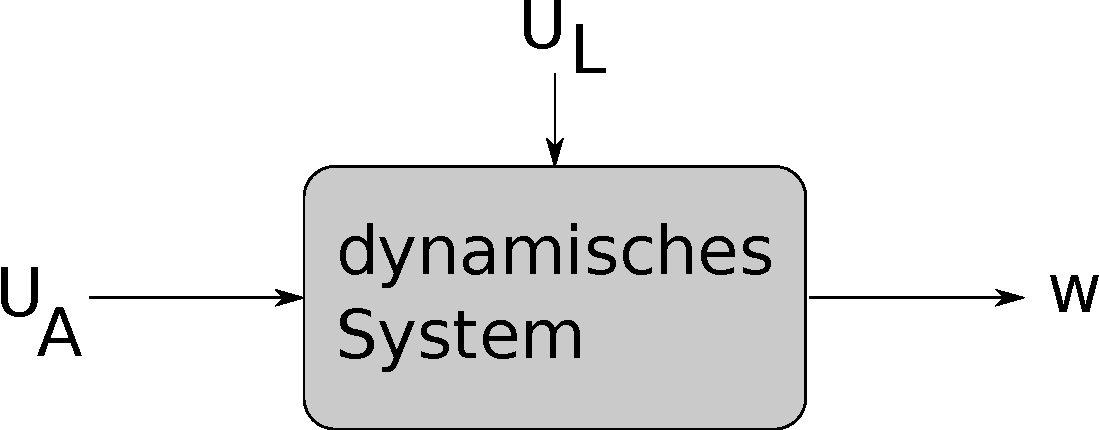
\includegraphics[width=200px]{graphics/gleichstrommotor.pdf}
\end{center}

\subsubsection{Ermittlung der beschreibenden Gleichungen:}

  \[u_l(t) = L \frac{di_A(t)} {dt} \longrightarrow \frac{d i_A(t)}{dt} = \frac{1}{L_A} u_l(t) \]
\begin{equation}
   \xrightarrow {\text{Integration von 0 bis t}} i_A(t) = i_A(0) + \frac{1}{L_A} \int_0^t u_l(\tau), d \tau 
\end{equation}
 \[u_A(t) = u_R + u_L + u_{ind} \]
\begin{equation}
\longrightarrow u_L(t) = u_A(t) - u_R(t) - u_{ind}(t)
\end{equation}

\begin{equation}
 u_R(t) = R_A i_A(t)
\end{equation}

\begin{equation}
 u_{ind}(t) = c \phi_F \omega(t)
\end{equation}

\subsubsection*{rotierender Anker + Welle:}
\[J\dot{\omega} = M_\Sigma
\longrightarrow \dot{\omega} = \frac{1}{J} M_\Sigma(t) \]
\begin{equation}
 \xrightarrow {\text{Integration von 0 bis t}}  \omega(t) = \omega(0) + \frac{1}{J} \int_0^t M_z(\tau), d \tau
\end{equation}










=======
=======
>>>>>>> 5146e1967d6928da3c6b0ee572d465bc5b52ef94:content/modellbildung.tex
=======
>>>>>>> 5146e1967d6928da3c6b0ee572d465bc5b52ef94:content/modellbildung.tex
		\begin{center}
			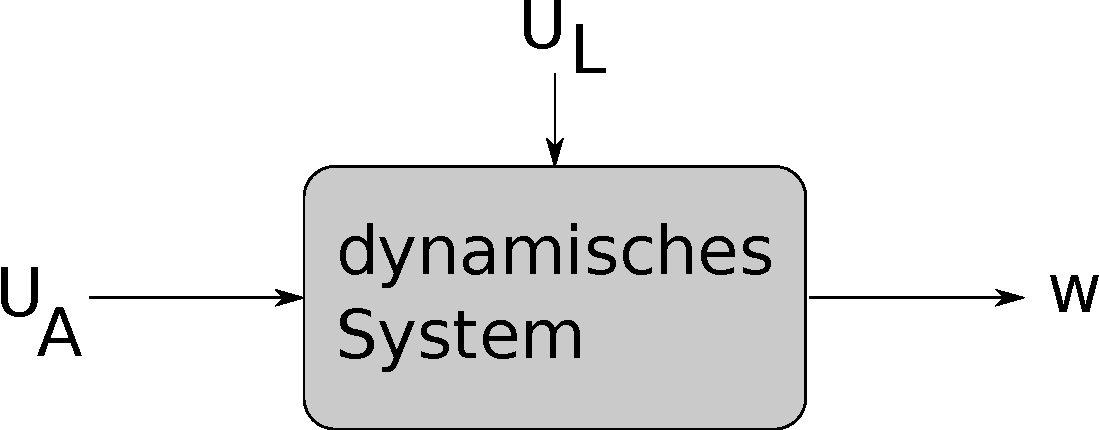
\includegraphics[width=200px]{graphics/gleichstrommotor.pdf}
		\end{center}
	\item Ermittlung der beschreibenden Gleichungen
		\subitem Ankerstromkreis
		\begin{align}
		u_L=L\frac{di_A}{dt} \rightarrow \frac{di_A(t)}{dt}=\frac{1}{L}u_L(t) \stackrel{\int_0^t}{\rightarrow}i_A(t)=i_A(0)+\frac{1}{L_A}\int_0^t u_L(\tau)d\tau \\
		u_A=u_R+u_L+u_{ind} \rightarrow u_L(t)=u_A(t)-u_R(t)-u_{ind}(t) \\
		u_R(t)=R_Ai_A(t) \\
		U_{ind}=c\phi\omega(t)
		\end{align}
		\subitem Rotierender Anker und Welle
		\begin{align}
		J\dot{\omega}=M_{\sum} \rightarrow \dot{\omega}(t)=\frac{1}{J}M_{\sum}(t)\stackrel{\int_0^t}{\rightarrow}\omega(t)=\omega(0)+\frac{1}{J}\int_0^t M_{\sum}(\tau)d\tau \\
		M_{\sum}(t)=M_A(t)-M_L(t) \\
		M_A(t) = c \phi_F L_A(t)
		\end{align}
	\item �bersetzung der Gleichungen ins Strukturbild {TODO:BILD}
<<<<<<< HEAD:content/modellbildung.tex
<<<<<<< HEAD:content/modellbildung.tex
\end{itemize}
>>>>>>> 5146e1967d6928da3c6b0ee572d465bc5b52ef94:content/modellbildung.tex
=======
\end{itemize}
>>>>>>> 5146e1967d6928da3c6b0ee572d465bc5b52ef94:content/modellbildung.tex
=======
\end{itemize}
>>>>>>> 5146e1967d6928da3c6b0ee572d465bc5b52ef94:content/modellbildung.tex
